\documentclass[11pt,a4paper]{report}
\usepackage[textwidth=37em,vmargin=30mm]{geometry}
\usepackage{calc,xunicode,amsmath,amssymb,paralist,enumitem,tabu,booktabs,datetime2,xeCJK,xeCJKfntef,listings}
\usepackage{tocloft,fancyhdr,tcolorbox,xcolor,graphicx,eso-pic,xltxtra,xelatexemoji}

\newcommand{\envyear}[0]{2025}
\newcommand{\envdatestr}[0]{2025-02-12}
\newcommand{\envfinaldir}[0]{webdb/2025/20250212/final}

\usepackage[hidelinks]{hyperref}
\hypersetup{
    colorlinks=false,
    pdfpagemode=FullScreen,
    pdftitle={Web Digest - \envdatestr}
}

\setlength{\cftbeforechapskip}{10pt}
\renewcommand{\cftchapfont}{\rmfamily\bfseries\large\raggedright}
\setlength{\cftbeforesecskip}{2pt}
\renewcommand{\cftsecfont}{\sffamily\small\raggedright}

\setdefaultleftmargin{2em}{2em}{1em}{1em}{1em}{1em}

\usepackage{xeCJK,xeCJKfntef}
\xeCJKsetup{PunctStyle=plain,RubberPunctSkip=false,CJKglue=\strut\hskip 0pt plus 0.1em minus 0.05em,CJKecglue=\strut\hskip 0.22em plus 0.2em}
\XeTeXlinebreaklocale "zh"
\XeTeXlinebreakskip = 0pt


\setmainfont{Brygada 1918}
\setromanfont{Brygada 1918}
\setsansfont{IBM Plex Sans}
\setmonofont{JetBrains Mono NL}
\setCJKmainfont{Noto Serif CJK SC}
\setCJKromanfont{Noto Serif CJK SC}
\setCJKsansfont{Noto Sans CJK SC}
\setCJKmonofont{Noto Sans CJK SC}

\setlength{\parindent}{0pt}
\setlength{\parskip}{8pt}
\linespread{1.15}

\lstset{
	basicstyle=\ttfamily\footnotesize,
	numbersep=5pt,
	backgroundcolor=\color{black!5},
	showspaces=false,
	showstringspaces=false,
	showtabs=false,
	tabsize=2,
	captionpos=b,
	breaklines=true,
	breakatwhitespace=true,
	breakautoindent=true,
	linewidth=\textwidth
}






\newcommand{\coverpic}[2]{
    % argv: itemurl, authorname
    Cover photo by #2~~(\href{#1}{#1})
}
\newcommand{\makeheader}[0]{
    \begin{titlepage}
        % \newgeometry{hmargin=15mm,tmargin=21mm,bmargin=12mm}
        \begin{center}
            
            \rmfamily\scshape
            \fontspec{BaskervilleF}
            \fontspec{Old Standard}
            \fontsize{59pt}{70pt}\selectfont
            WEB\hfill DIGEST
            
            \vfill
            % \vskip 30pt
            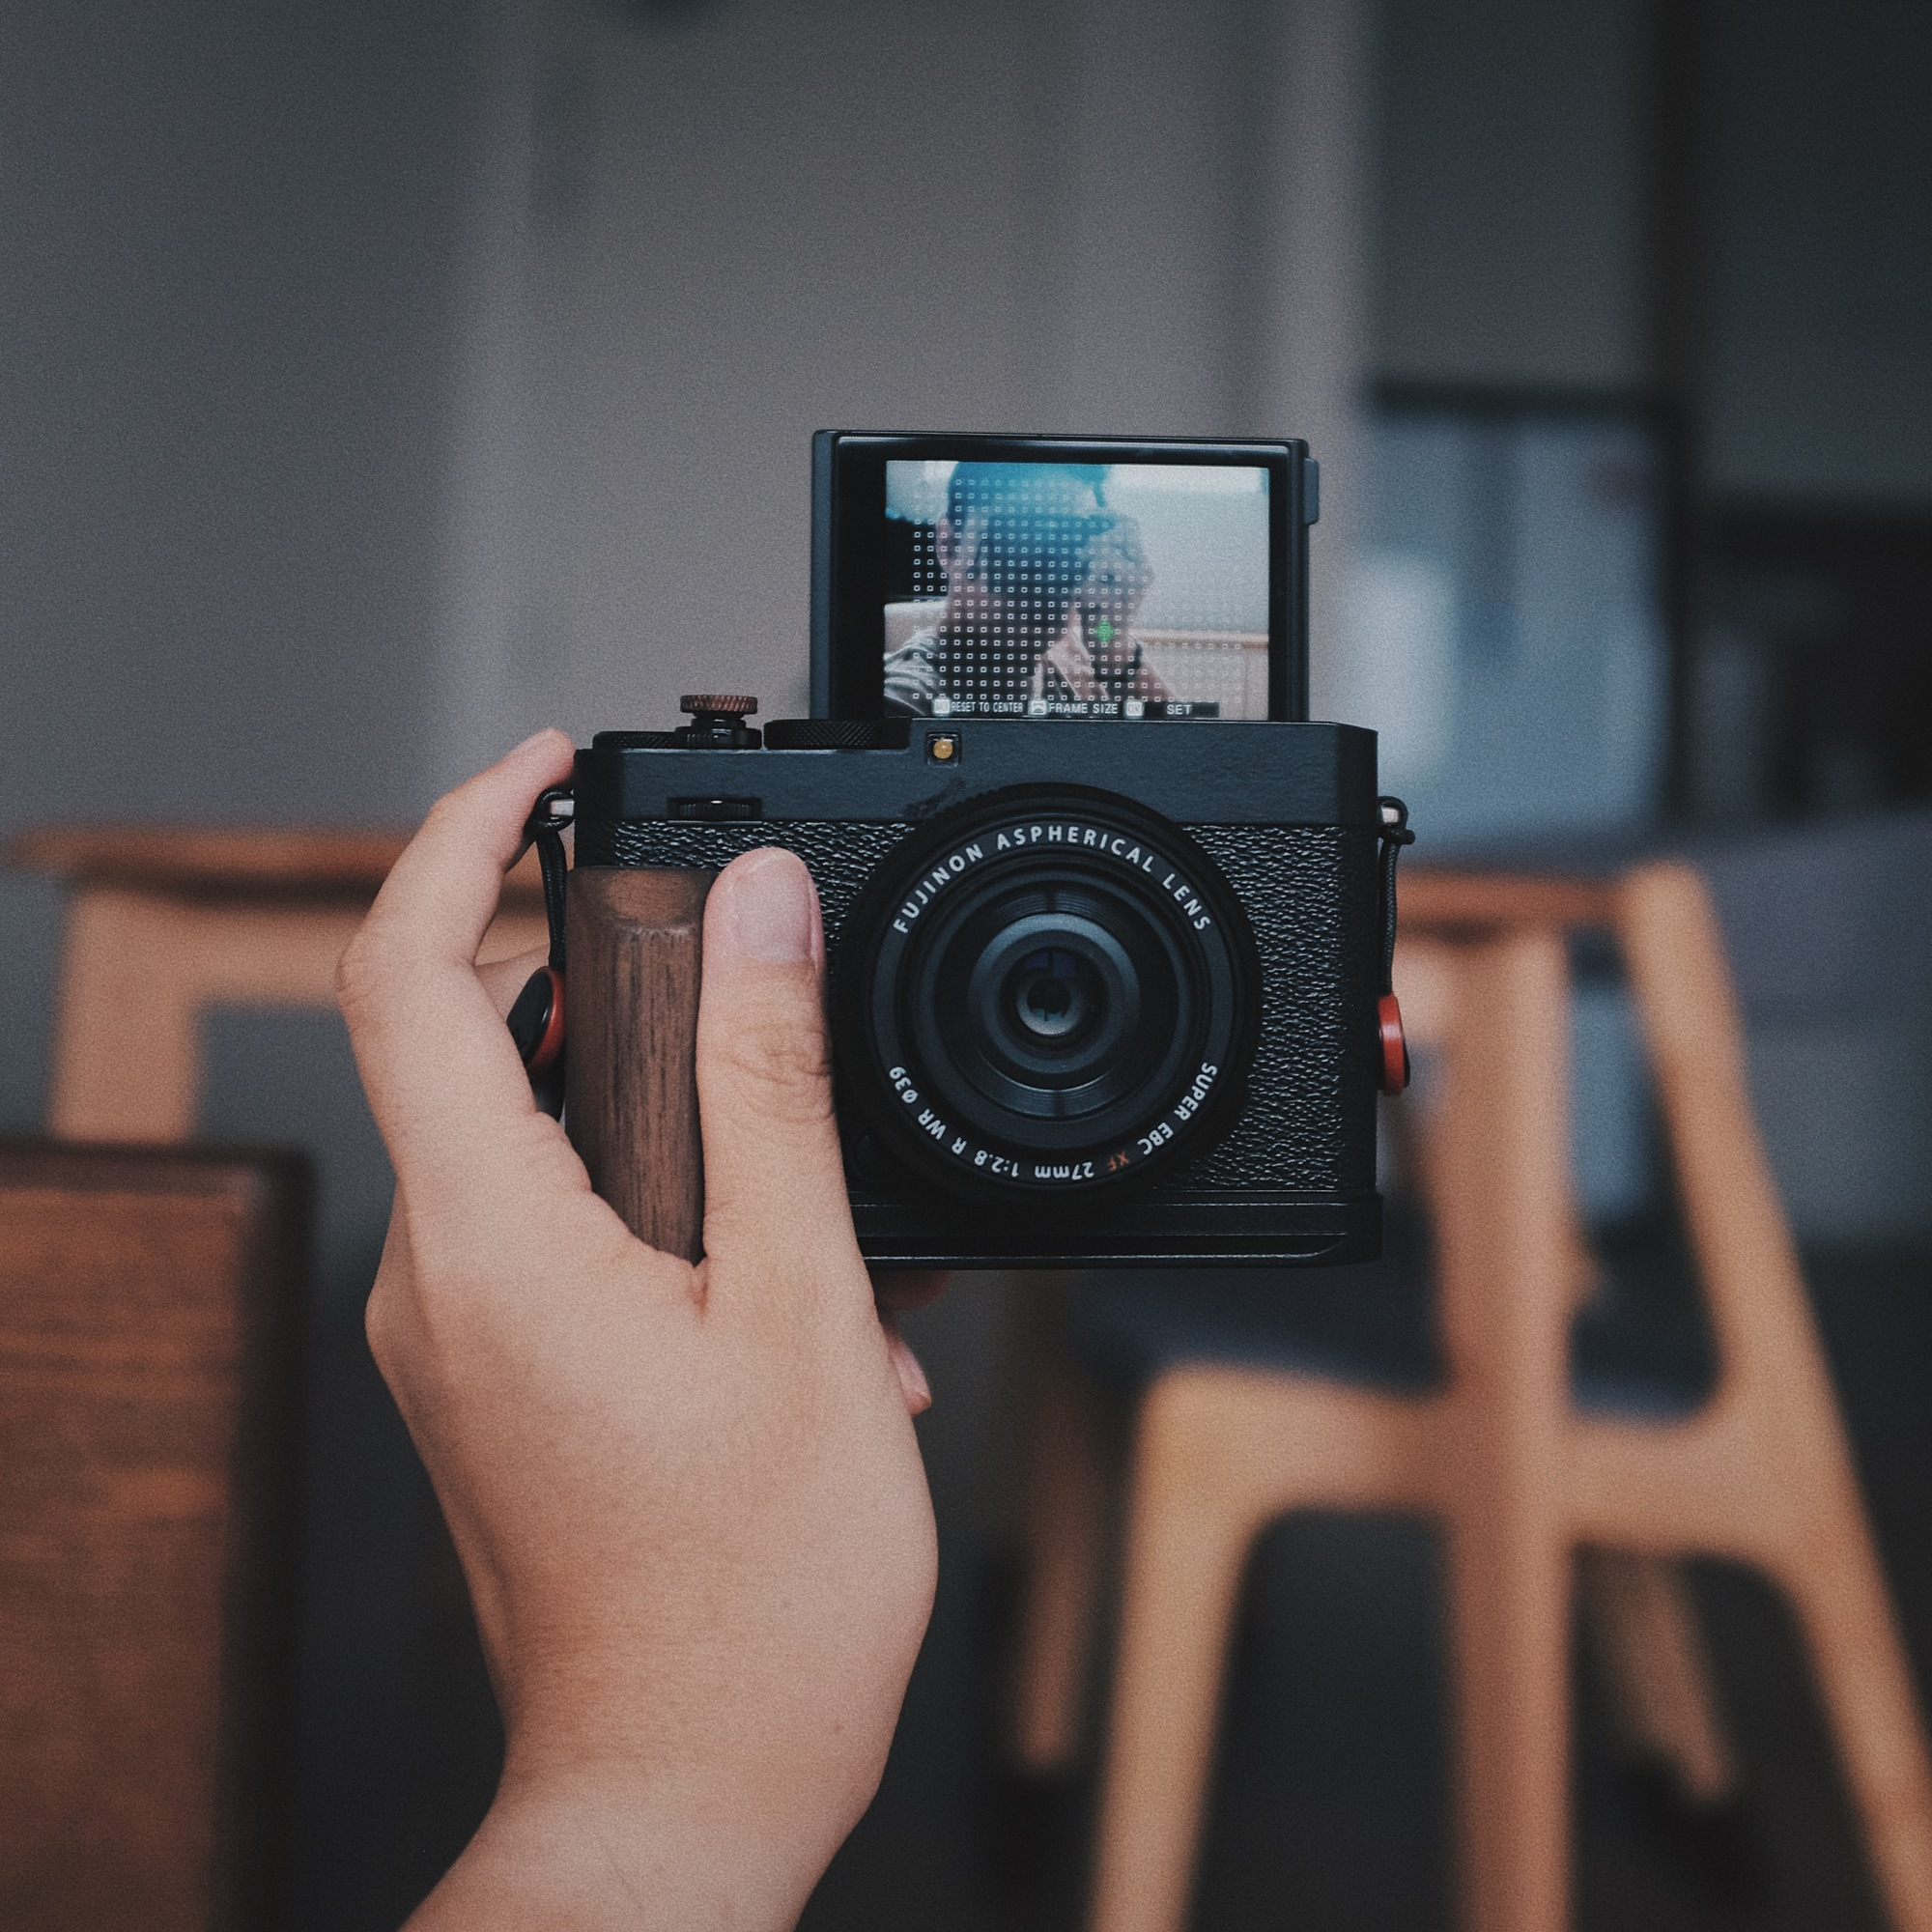
\includegraphics[width=\linewidth]{\envfinaldir/coverpic-prod.jpg}\par
            % \vskip 30pt
            \vfill

            \normalsize\rmfamily\scshape
            \copyright{} The Web Digest Project \hfill\large \envdatestr
        \end{center}
    \end{titlepage}
    % \restoregeometry
}
\newcommand{\simplehref}[1]{%
    \textcolor{blue!80!green}{\href{#1}{#1}}%
}
\renewcommand{\contentsname}{\center\Huge\sffamily\bfseries Contents\par\vskip 20pt}
\newcounter{ipartcounter}
\setcounter{ipartcounter}{0}
\newcommand{\ipart}[1]{
    % \vskip 20pt
    \clearpage
    \stepcounter{ipartcounter}
    \phantomsection
    \addcontentsline{toc}{chapter}{#1}
    % \begin{center}
    %     \Huge
    %     \sffamily\bfseries
    %     #1
    % \end{center}
    % \vskip 20pt plus 7pt
}
\newcounter{ichaptercounter}
\setcounter{ichaptercounter}{0}
\newcommand{\ichapter}[1]{
    % \vskip 20pt
    \clearpage
    \stepcounter{ichaptercounter}
    \phantomsection
    \addcontentsline{toc}{section}{\numberline{\arabic{ichaptercounter}}#1}
    \begin{center}
        \Huge
        \sffamily\bfseries
        #1
    \end{center}
    \vskip 20pt plus 7pt
}
\newcommand{\entrytitlefont}[1]{\subsection*{\raggedright\Large\sffamily\bfseries#1}}
\newcommand{\entryitemGeneric}[2]{
    % argv: title, url
    \parbox{\linewidth}{
        \entrytitlefont{#1}\par\vskip 5pt
        \footnotesize\ttfamily\mdseries
        \simplehref{#2}
    }\vskip 11pt plus 11pt minus 1pt
}
\newcommand{\entryitemGithub}[3]{
    % argv: title, url, desc
    \parbox{\linewidth}{
        \entrytitlefont{#1}\par\vskip 5pt
        \footnotesize\ttfamily\mdseries
        \simplehref{#2}\par\vskip 5pt
        \small\rmfamily\mdseries#3
    }\vskip 11pt plus 11pt minus 1pt
}
\newcommand{\entryitemAp}[3]{
    % argv: title, url, desc
    \parbox{\linewidth}{
        \entrytitlefont{#1}\par\vskip 5pt
        \footnotesize\ttfamily\mdseries
        \simplehref{#2}\par\vskip 5pt
        \small\rmfamily\mdseries#3
    }\vskip 11pt plus 11pt minus 1pt
}
\newcommand{\entryitemHackernews}[3]{
    % argv: title, hnurl, rawurl
    % \parbox{\linewidth}{
    %     \entrytitlefont{#1}\par\vskip 5pt
    %     \footnotesize\ttfamily\mdseries
    %     \simplehref{#3}\par
    %     \textcolor{black!50}{\href{#2}{#2}}
    % }\vskip 11pt plus 11pt minus 1pt
    \begin{minipage}{\linewidth}
            \entrytitlefont{#1}\par\vskip 5pt
            \footnotesize\ttfamily\mdseries
            \simplehref{#3}\par
            \textcolor{black!50}{\href{#2}{#2}}
    \end{minipage}\par\vskip 11pt plus 11pt minus 1pt
}







\begin{document}

\makeheader

\tableofcontents\clearpage




\ipart{Developers}
\ichapter{Hacker News}
\entryitemTwoLinks{Thomson Reuters wins first major AI copyright case in the US}{https://news.ycombinator.com/item?id=43018251}{https://www.wired.com/story/thomson-reuters-ai-copyright-lawsuit/}

\entryitemTwoLinks{DeepScaleR: Surpassing O1-Preview with a 1.5B Model by Scaling RL}{https://news.ycombinator.com/item?id=43017599}{https://pretty-radio-b75.notion.site/DeepScaleR-Surpassing-O1-Preview-with-a-1-5B-Model-by-Scaling-RL-19681902c1468005bed8ca303013a4e2}

\entryitemTwoLinks{The subtle art of designing physical controls for cars}{https://news.ycombinator.com/item?id=43017010}{https://www.theturnsignalblog.com/the-subtle-art-of-designing-physical-control-for-cars/}

\entryitemTwoLinks{Tesla Cybertruck Drives Itself into a Pole, Owner Says 'Thank You Tesla'}{https://news.ycombinator.com/item?id=43016931}{https://www.thedrive.com/news/tesla-cybertruck-drove-itself-into-a-pole-owner-says-thank-you-tesla}

\entryitemTwoLinks{UnitedHealth hired a defamation law firm to go after social media posts}{https://news.ycombinator.com/item?id=43015713}{https://fortune.com/2025/02/10/unitedhealth-defamation-law-firm-social-media/}

\entryitemTwoLinks{IT Unemployment Rises to 5.7\% as AI Hits Tech Jobs}{https://news.ycombinator.com/item?id=43015397}{https://www.wsj.com/articles/it-unemployment-rises-to-5-7-as-ai-hits-tech-jobs-7726bb1b}

\entryitemTwoLinks{Launch HN: A0.dev (YC W25) – React Native App Generator}{https://news.ycombinator.com/item?id=43015267}{https://news.ycombinator.com/item?id=43015267}

\entryitemTwoLinks{LLMs can teach themselves to better predict the future}{https://news.ycombinator.com/item?id=43014918}{https://arxiv.org/abs/2502.05253}

\entryitemTwoLinks{Intel's Battlemage Architecture}{https://news.ycombinator.com/item?id=43014408}{https://chipsandcheese.com/p/intels-battlemage-architecture}

\entryitemTwoLinks{I tasted Honda's spicy rodent-repelling tape and I will do it again (2021)}{https://news.ycombinator.com/item?id=43013615}{https://haterade.substack.com/p/i-tasted-hondas-spicy-rodent-repelling}

\entryitemTwoLinks{Backblaze Drive Stats for 2024}{https://news.ycombinator.com/item?id=43013431}{https://www.backblaze.com/blog/backblaze-drive-stats-for-2024/}

\entryitemTwoLinks{Boring tech is mature, not old}{https://news.ycombinator.com/item?id=43012862}{https://rubenerd.com/boring-tech-is-mature-not-old/}

\entryitemTwoLinks{FLAC 1.5 Delivers Multi-Threaded Encoding}{https://news.ycombinator.com/item?id=43012751}{https://www.phoronix.com/news/FLAC-1.5-Released}

\entryitemTwoLinks{Microsoft open sources PostgreSQL extensions}{https://news.ycombinator.com/item?id=43012294}{https://www.theregister.com/2025/02/11/microsoft\_postgresql\_extensions/}

\entryitemTwoLinks{Firing programmers for AI is a mistake}{https://news.ycombinator.com/item?id=43010814}{https://defragzone.substack.com/p/techs-dumbest-mistake-why-firing}

\entryitemTwoLinks{How about trailing commas in SQL?}{https://news.ycombinator.com/item?id=43010365}{http://peter.eisentraut.org/blog/2025/02/11/how-about-trailing-commas-in-sql}

\entryitemTwoLinks{Working from home is here to stay}{https://news.ycombinator.com/item?id=43010037}{https://wolfstreet.com/2025/02/10/there-hasnt-been-much-if-any-reduction-in-wfh-in-over-2-years-despite-all-the-hype-about-rto/}

\entryitemTwoLinks{TSMC 2nm Process Disclosure – How Does It Measure Up?}{https://news.ycombinator.com/item?id=43009850}{https://semiwiki.com/semiconductor-services/techinsights/352972-iedm-2025-tsmc-2nm-process-disclosure-how-does-it-measure-up/}

\entryitemTwoLinks{Jeep Introduces Pop-Up Ads That Appear Every Time You Stop}{https://news.ycombinator.com/item?id=43009682}{https://tech.slashdot.org/story/25/02/11/0016258/jeep-introduces-pop-up-ads-that-appear-every-time-you-stop}

\entryitemTwoLinks{Meta's Hyperscale Infrastructure: Overview and Insights}{https://news.ycombinator.com/item?id=43008920}{https://cacm.acm.org/research/metas-hyperscale-infrastructure-overview-and-insights/}\ichapter{Phoronix}
\entryitemGeneric{\hskip 0pt{}Python 3.14 Alpha 5 Released With New Tail-Call Interpreter}{https://www.phoronix.com/news/Python-3.14-Alpha-5}

\entryitemGeneric{\hskip 0pt{}Healthy Competition With GCC 15 vs. LLVM Clang 20 Performance On AMD Zen 5}{https://www.phoronix.com/review/clang20-gcc15-amd-znver5}

\entryitemGeneric{\hskip 0pt{}Intel CPU Microcode Updated For Five New Security Issues}{https://www.phoronix.com/news/Intel-Microcode-20250211}

\entryitemGeneric{\hskip 0pt{}GNOME 48 Now Allows Grouping Notifications By App}{https://www.phoronix.com/news/GNOME-48-Notifications-App}

\entryitemGeneric{\hskip 0pt{}Ubuntu 25.04's GNOME Web Browser Will Be Able To Play More Web Videos By Default}{https://www.phoronix.com/news/Ubuntu-Epiphany-Bad-Plugins}

\entryitemGeneric{\hskip 0pt{}Arm Mali Panfrost Driver Lands OpenCL C Support In Mesa 25.1}{https://www.phoronix.com/news/Panfrost-Lands-OpenCL-C}

\entryitemGeneric{\hskip 0pt{}FLAC 1.5 Finally Delivers Multi-Threaded Encoding}{https://www.phoronix.com/news/FLAC-1.5-Released}

\entryitemGeneric{\hskip 0pt{}KDE Plasma 6.3 Released With Improved Fractional Scaling \& Other Enhancements}{https://www.phoronix.com/news/KDE-Plasma-6.3-Released}

\entryitemGeneric{\hskip 0pt{}AMD AOMP 20.0-2 Compiler Adds The "flang-new" Fortran Compiler Option}{https://www.phoronix.com/news/AMD-AOMP-20.0-2}\ichapter{Dribbble}
\entryitemGeneric{\hskip 0pt{}Self Love}{https://dribbble.com/shots/25607914-Self-Love}

\entryitemGeneric{\hskip 0pt{}Urban Echo}{https://dribbble.com/shots/25608526-Urban-Echo}

\entryitemGeneric{\hskip 0pt{}Cloaked Wireless Device}{https://dribbble.com/shots/25403560-Cloaked-Wireless-Device}

\entryitemGeneric{\hskip 0pt{}Logo tip 001. Symmetry and asymmetry}{https://dribbble.com/shots/25606111-Logo-tip-001-Symmetry-and-asymmetry}

\entryitemGeneric{\hskip 0pt{}Sentinal - Logo Design}{https://dribbble.com/shots/25606497-Sentinal-Logo-Design}

\entryitemGeneric{\hskip 0pt{}Tanuki}{https://dribbble.com/shots/25606258-Tanuki}

\entryitemGeneric{\hskip 0pt{}Barbershop POS app for booking and payments}{https://dribbble.com/shots/25596116-Barbershop-POS-app-for-booking-and-payments}

\entryitemGeneric{\hskip 0pt{}Seam Logo Redesigned}{https://dribbble.com/shots/25595119-Seam-Logo-Redesigned}

\entryitemGeneric{\hskip 0pt{}HugNecks®}{https://dribbble.com/shots/25596356-HugNecks}

\entryitemGeneric{\hskip 0pt{}Payoneer App Concept Design}{https://dribbble.com/shots/25593820-Payoneer-App-Concept-Design}

\entryitemGeneric{\hskip 0pt{}Nimmio}{https://dribbble.com/shots/25594035-Nimmio}

\entryitemGeneric{\hskip 0pt{}Aphmau Cat}{https://dribbble.com/shots/25593493-Aphmau-Cat}

\entryitemGeneric{\hskip 0pt{}Playtech Animated Icons - Payments}{https://dribbble.com/shots/25592523-Playtech-Animated-Icons-Payments}

\entryitemGeneric{\hskip 0pt{}Cloaked Logo Design}{https://dribbble.com/shots/25585116-Cloaked-Logo-Design}

\entryitemGeneric{\hskip 0pt{}CropBytes 2d \& 3d logo}{https://dribbble.com/shots/25590388-CropBytes-2d-3d-logo}

\entryitemGeneric{\hskip 0pt{}The Journey}{https://dribbble.com/shots/25590279-The-Journey}

\entryitemGeneric{\hskip 0pt{}Easyalgos Logo Design}{https://dribbble.com/shots/25589439-Easyalgos-Logo-Design}

\entryitemGeneric{\hskip 0pt{}Tailor Brands Logo}{https://dribbble.com/shots/25590868-Tailor-Brands-Logo}

\entryitemGeneric{\hskip 0pt{}Wylder Logo Design - W letter monogram}{https://dribbble.com/shots/25589195-Wylder-Logo-Design-W-letter-monogram}

\entryitemGeneric{\hskip 0pt{}Playtech Animated Icons - FAQ}{https://dribbble.com/shots/25586586-Playtech-Animated-Icons-FAQ}

\entryitemGeneric{\hskip 0pt{}Carbon Solutions B2B Branding Design \& Visual Identity}{https://dribbble.com/shots/25525140-Carbon-Solutions-B2B-Branding-Design-Visual-Identity}

\entryitemGeneric{\hskip 0pt{}Frank's Alley® Trailer \& Mascots}{https://dribbble.com/shots/25585516-Frank-s-Alley-Trailer-Mascots}

\entryitemGeneric{\hskip 0pt{}Dog / Puzzle Logo}{https://dribbble.com/shots/25581316-Dog-Puzzle-Logo}

\entryitemGeneric{\hskip 0pt{}Glyph Beer Icons 51-62}{https://dribbble.com/shots/25585199-Glyph-Beer-Icons-51-62}


\ipart{Developers~~~~(zh-Hans)}
\ichapter{Solidot}
\entryitemGeneric{\hskip 0pt{}DeepSeek AI 训练成本并不低}{https://www.solidot.org/story?sid=80531}

\entryitemGeneric{\hskip 0pt{}上海自研 GLP-1 糖尿病新药批准上市}{https://www.solidot.org/story?sid=80530}

\entryitemGeneric{\hskip 0pt{}微软研究发现 AI 可能会导致人类认知能力退化}{https://www.solidot.org/story?sid=80529}

\entryitemGeneric{\hskip 0pt{}美国优秀 AI 人才四成来自中国}{https://www.solidot.org/story?sid=80528}

\entryitemGeneric{\hskip 0pt{}OpenAI 预计数个月内完成自研 AI 芯片的设计}{https://www.solidot.org/story?sid=80527}

\entryitemGeneric{\hskip 0pt{}对国内大学生的研究发现锻炼有助于减轻网瘾症状}{https://www.solidot.org/story?sid=80526}

\entryitemGeneric{\hskip 0pt{}科学家发现宇宙最大结构 Quipu}{https://www.solidot.org/story?sid=80525}

\entryitemGeneric{\hskip 0pt{}感染 COVID-19 可能加速大脑衰老四年}{https://www.solidot.org/story?sid=80524}

\entryitemGeneric{\hskip 0pt{}地球内核并非完全固态}{https://www.solidot.org/story?sid=80523}

\entryitemGeneric{\hskip 0pt{}TikTok 鼓励美国 Android 用户通过其官网下载 APK}{https://www.solidot.org/story?sid=80522}

\entryitemGeneric{\hskip 0pt{}癌症疫苗让小鼠恢复活力但会对人类有效吗?}{https://www.solidot.org/story?sid=80521}

\entryitemGeneric{\hskip 0pt{}Aaron Swartz 雕像在互联网档案馆揭幕}{https://www.solidot.org/story?sid=80520}

\entryitemGeneric{\hskip 0pt{}欧几里得望远镜捕捉到完美爱因斯坦环}{https://www.solidot.org/story?sid=80518}

\entryitemGeneric{\hskip 0pt{}月球南极附近的两条大峡谷是在不到 10 分钟内形成的}{https://www.solidot.org/story?sid=80517}

\entryitemGeneric{\hskip 0pt{}LibreOffice 25.2 释出}{https://www.solidot.org/story?sid=80516}

\entryitemGeneric{\hskip 0pt{}工作、自愿服务和文字游戏等有助于改善老年人的认知}{https://www.solidot.org/story?sid=80515}

\entryitemGeneric{\hskip 0pt{}大脑微塑料浓度高于其他器官}{https://www.solidot.org/story?sid=80514}

\entryitemGeneric{\hskip 0pt{}如何让 AMD Zen CPU 总是生成 4 作为随机数}{https://www.solidot.org/story?sid=80513}

\entryitemGeneric{\hskip 0pt{}reCAPTCHA 变成了 Google 的间谍软件}{https://www.solidot.org/story?sid=80512}

\entryitemGeneric{\hskip 0pt{}科学家揭示螳螂虾如何在不损伤自身的情况下拳击猎物}{https://www.solidot.org/story?sid=80511}\ichapter{V2EX}
\entryitemGeneric{\hskip 0pt{}[macOS] Mac 上切换应用真的烦死人。}{https://www.v2ex.com/t/1110811}

\entryitemGeneric{\hskip 0pt{}[宽带症候群] DeepSeek 推荐我购买 22/23 AWG 规格的 Cat 6A 线,但是我找不到 22/23 AWG 规格的成品网线}{https://www.v2ex.com/t/1110810}

\entryitemGeneric{\hskip 0pt{}[问与答] 看到 MBI 的消息有感}{https://www.v2ex.com/t/1110809}

\entryitemGeneric{\hskip 0pt{}[游戏开发] 为什么 Unity 的编译速度会这么离谱?真的是 Mono 的问题吗?}{https://www.v2ex.com/t/1110808}

\entryitemGeneric{\hskip 0pt{}[分享发现] [AI] 发现一个新的便宜 AI API 平台}{https://www.v2ex.com/t/1110807}

\entryitemGeneric{\hskip 0pt{}[酷工作] 招聘 Java 开发工程师 [9-29k]}{https://www.v2ex.com/t/1110805}

\entryitemGeneric{\hskip 0pt{}[分享创造] alipan backup 备份文件到阿里云盘 | 跨平台}{https://www.v2ex.com/t/1110804}

\entryitemGeneric{\hskip 0pt{}[VXNA] 申请收录: Shaun's Space}{https://www.v2ex.com/t/1110803}

\entryitemGeneric{\hskip 0pt{}[Flutter] 有 flutter 大佬么?请教几个问题}{https://www.v2ex.com/t/1110802}

\entryitemGeneric{\hskip 0pt{}[Chrome] FetchImage:一键提取网页图片的 Chrome 扩展,效率翻倍!求支持!}{https://www.v2ex.com/t/1110801}

\entryitemGeneric{\hskip 0pt{}[游戏开发] Unity 裁员把刚加的决策树又干没了, Unity 7 的大饼很可能也没了。}{https://www.v2ex.com/t/1110800}

\entryitemGeneric{\hskip 0pt{}[程序员] js-screen-shot 插件修复在高分屏上的模糊问题~}{https://www.v2ex.com/t/1110799}

\entryitemGeneric{\hskip 0pt{}[天黑以后] 20250212 午夜俱乐部}{https://www.v2ex.com/t/1110798}

\entryitemGeneric{\hskip 0pt{}[程序员] 请问训练或者调试 yolo 用什么配置性价比较高。}{https://www.v2ex.com/t/1110797}

\entryitemGeneric{\hskip 0pt{}[投资] 你们身边有接触过真实存在的牛散吗}{https://www.v2ex.com/t/1110796}

\entryitemGeneric{\hskip 0pt{}[分享创造] 烦了很久的 cursor markdown 代码块转义混乱问题 ! 写 prompt 解决了}{https://www.v2ex.com/t/1110795}

\entryitemGeneric{\hskip 0pt{}[问与答] 被一个固定邮箱发邮件骚扰,你会怎么办}{https://www.v2ex.com/t/1110793}

\entryitemGeneric{\hskip 0pt{}[程序员] 技术栈基础设施选型}{https://www.v2ex.com/t/1110791}

\entryitemGeneric{\hskip 0pt{}[职场话题] 八年前端分享最近两周面试情况}{https://www.v2ex.com/t/1110790}

\entryitemGeneric{\hskip 0pt{}[Mac mini] 狗东国补买的 Mac Mini 到手以后发现 Power Cycles 有 120 多,是翻车了吗?}{https://www.v2ex.com/t/1110789}

\entryitemGeneric{\hskip 0pt{}[Apple] 苹果与阿里巴巴合作开发人工智能}{https://www.v2ex.com/t/1110788}

\entryitemGeneric{\hskip 0pt{}[问与答] 現在相對(最)好用的 AI 模型是哪個?}{https://www.v2ex.com/t/1110786}

\entryitemGeneric{\hskip 0pt{}[宽带症候群] 寻找性价比高的一次性流量包推荐}{https://www.v2ex.com/t/1110785}

\entryitemGeneric{\hskip 0pt{}[电影] 哪吒 120 亿,饺子导演能分 到 20 亿吗?}{https://www.v2ex.com/t/1110784}

\entryitemGeneric{\hskip 0pt{}[Cloudflare] 大家有使用 cloudflare 的 R2 的吗?}{https://www.v2ex.com/t/1110783}

\entryitemGeneric{\hskip 0pt{}[问与答] 大家有啥长期使用并安利的软件}{https://www.v2ex.com/t/1110782}

\entryitemGeneric{\hskip 0pt{}[Apple] 消息称苹果测试了 DeepSeek 模型但没有继续使用,最终将联手阿里巴巴为中国 iPhone 用户提供 AI 功能}{https://www.v2ex.com/t/1110781}

\entryitemGeneric{\hskip 0pt{}[骑行] 日常通勤往返 5km,小白求推荐一辆自行车,预算最好控制在 3500 元以内。}{https://www.v2ex.com/t/1110780}

\entryitemGeneric{\hskip 0pt{}[分享创造] 做了一个限制刷手机的安卓 APP}{https://www.v2ex.com/t/1110779}

\entryitemGeneric{\hskip 0pt{}[生活] 分享一篇文章``原生家庭如何影响婚姻关系''}{https://www.v2ex.com/t/1110778}

\entryitemGeneric{\hskip 0pt{}[京东] 山姆会员卡激活时如果不是 11 位手机号(港澳号码)就无法和京东绑定}{https://www.v2ex.com/t/1110777}

\entryitemGeneric{\hskip 0pt{}[宽带症候群] OP 路由禁止 IPv6 解析,但手机微信仍在跑 IPv6 流量}{https://www.v2ex.com/t/1110776}

\entryitemGeneric{\hskip 0pt{}[Telegram] 请问现在最低成本注册登录 Telegram 的方法是哪种?}{https://www.v2ex.com/t/1110775}

\entryitemGeneric{\hskip 0pt{}[程序员] 寻求技术支持搭建 GitHub 上的 AstrBot 机器人 项目(报酬有限,兴趣优先)}{https://www.v2ex.com/t/1110774}

\entryitemGeneric{\hskip 0pt{}[宽带症候群] 武汉电信 可以申请 5g 599 2000M 上传 500M 宽带}{https://www.v2ex.com/t/1110773}

\entryitemGeneric{\hskip 0pt{}[Minecraft] 快点 Minecraft 服务器 一起来玩吧~}{https://www.v2ex.com/t/1110772}

\entryitemGeneric{\hskip 0pt{}[问与答] @Livid. 提个建议.关于回复乱套}{https://www.v2ex.com/t/1110771}

\entryitemGeneric{\hskip 0pt{}[NAS] nas 支持远程触发下载任务吗}{https://www.v2ex.com/t/1110769}

\entryitemGeneric{\hskip 0pt{}[Apple] [紧急求助‼️] macOS 15.x 下 AirDrop 突然文件丢失,求助各路大神}{https://www.v2ex.com/t/1110768}

\entryitemGeneric{\hskip 0pt{}[求职] [北京] 4 年 Java 求职}{https://www.v2ex.com/t/1110767}

\entryitemGeneric{\hskip 0pt{}[分享创造] 分享自己弄的一个 Hugo 主题: hugo-theme-deck}{https://www.v2ex.com/t/1110766}

\entryitemGeneric{\hskip 0pt{}[分享发现] Huke T3 触摸板测试}{https://www.v2ex.com/t/1110765}

\entryitemGeneric{\hskip 0pt{}[上海] [租房咨询] 普陀区曹杨路附近}{https://www.v2ex.com/t/1110764}

\entryitemGeneric{\hskip 0pt{}[问与答] 在哪里看编程能力模型的排名?}{https://www.v2ex.com/t/1110763}

\entryitemGeneric{\hskip 0pt{}[问与答] 有什么好用的多驱动管理软件吗}{https://www.v2ex.com/t/1110762}

\entryitemGeneric{\hskip 0pt{}[分享发现] 做了一个玩具:歌词编辑器}{https://www.v2ex.com/t/1110761}

\entryitemGeneric{\hskip 0pt{}[Bitcoin] 我 wise 账户中的余额,怎么可以换成比特币或是 USDT}{https://www.v2ex.com/t/1110760}

\entryitemGeneric{\hskip 0pt{}[Node.js] 请教大家一个在 hono.js 中使用 ts 的类型兼容性问题}{https://www.v2ex.com/t/1110759}

\entryitemGeneric{\hskip 0pt{}[问与答] iOS 上有什么不错的自动记账(配合捷径)app 么?}{https://www.v2ex.com/t/1110758}

\entryitemGeneric{\hskip 0pt{}[宽带症候群] 上海电信现在还能换不是 SDN 的网关吗}{https://www.v2ex.com/t/1110757}


\ipart{Generic News}
\ichapter{AP News}
\entryitemWithDescription{\hskip 0pt{}FBI says it found 2,400 new JFK assassination records}{https://apnews.com/article/0bd8ad5569f5fa3ed92b8ee9b795c9e7}{}

\entryitemWithDescription{\hskip 0pt{}A\$AP Rocky decides not to take the stand at his felony assault trial}{https://apnews.com/article/d727815dccc39150f80b10b90fd7eb1a}{}

\entryitemWithDescription{\hskip 0pt{}Kevin Hart will be the on-court emcee for Sunday's NBA All-Star tournament in San Francisco}{https://apnews.com/article/18b1ce7e347bb94f70aecc92723a8fd3}{}

\entryitemWithDescription{\hskip 0pt{}`Saturday Night Live' plans a massive 50th anniversary special. Who's coming and how to watch}{https://apnews.com/article/5f8001a3146e4602bc1d226f9224588d}{}

\entryitemWithDescription{\hskip 0pt{}Canned tuna sold at Trader Joe's, Costco, H-E-B recalled for botulism risk}{https://apnews.com/article/294f6ea8a347a84358715da5b6f16507}{}

\entryitemWithDescription{\hskip 0pt{}With metal detectors and patience, amateur treasure hunters unearth pieces of British history}{https://apnews.com/article/f1c71204cf142a6c8f5e9b16b998ba7d}{}

\entryitemWithDescription{\hskip 0pt{}Scientists say several thousand earthquakes detected near Greece's island of Santorini}{https://apnews.com/article/f3477a7000f547d2c6b3b5d797612a70}{}

\entryitemWithDescription{\hskip 0pt{}An unwanted double: US sales fall for American whiskeys as threats of a trade war heat up}{https://apnews.com/article/2988649c53240269a6df2a73ef8b3093}{}

\entryitemWithDescription{\hskip 0pt{}Philadelphia plans for a huge crowd to cheer on the Eagles at Super Bowl parade on Friday}{https://apnews.com/article/24eef77f33882c87e3aa5e54056e95b4}{}

\entryitemWithDescription{\hskip 0pt{}Roses are red, violets are blue, 940 million flowers are traveling (through Miami) to you}{https://apnews.com/article/a79c03ef5439b9473a7cd1f6c2fc24e6}{}

\entryitemWithDescription{\hskip 0pt{}Vince McMahon's lawyer was wrong to withhold documents sought by grand jury, court rules}{https://apnews.com/article/04c78ada42e765385e89afee8884e7eb}{}

\entryitemWithDescription{\hskip 0pt{}Trump signs order for plastic straws as he declares paper ones `don't work'}{https://apnews.com/article/e64e2671bbf7f8a8abaec0d5a491f7de}{}

\entryitemWithDescription{\hskip 0pt{}So long, penny! Trump orders US to ditch 1-cent coin after decades of complaints}{https://apnews.com/article/c4510debefe6cbfb0dd908d8fed7eb50}{}\ichapter{Reuters}
\entryitemWithDescription{\hskip 0pt{}NASA, SpaceX capsule swap to allow Starliner astronauts to return days sooner}{https://www.reuters.com/technology/space/nasa-spacex-capsule-swap-allow-starliner-astronauts-return-days-sooner-2025-02-11/}{NASA on Tuesday swapped out the astronaut capsule it plans to use for an upcoming routine flight to the International Space Station over SpaceX production delays, a scheduling move that allows for a slightly earlier return for the two...}

\entryitemWithDescription{\hskip 0pt{}Egypt plans to offer 'comprehensive proposal' to rebuild Gaza while Palestinians remain in Strip}{https://www.reuters.com/world/egypt-plans-offer-comprehensive-proposal-rebuild-gaza-while-palestinians-remain-2025-02-11/}{Egypt said on Tuesday it plans to offer a "comprehensive proposal" to rebuild Gaza while ensuring Palestinians remain on their land, according to a foreign ministry...}

\entryitemWithDescription{\hskip 0pt{}Egypt rejects allocating land to Gaza residents, state-affiliated TV says after Trump remarks}{https://www.reuters.com/world/egypt-rejects-allocating-land-gaza-residents-state-affiliated-tv-says-after-2025-02-11/}{Egypt rejected any proposal to allocate land to Gaza residents, the state-affiliated Al Qahera News TV reported on Tuesday, citing Egyptian...}

\entryitemWithDescription{\hskip 0pt{}Canada appoints new fentanyl czar to coordinate fight against smuggling}{https://www.reuters.com/world/americas/canada-appoints-new-fentanyl-czar-coordinate-fight-against-smuggling-2025-02-11/}{Canada, fulfilling a promise made to U.S. President Donald Trump, on Tuesday appointed a senior intelligence official to the new post of fentanyl czar, saying he would coordinate the fight against smuggling of the...}

\entryitemWithDescription{\hskip 0pt{}Musk takes aim at law firms involved in Trump policy challenges}{https://www.reuters.com/world/us/musk-takes-aim-law-firms-involved-trump-policy-challenges-2025-02-11/}{President Donald Trump\textquotesingle s billionaire ally Elon Musk on Tuesday directed his ire at U.S. law firms that have teamed up with advocacy groups to challenge the Republican\textquotesingle s sweeping policy changes in...}

\entryitemWithDescription{\hskip 0pt{}Trump pushes for use of plastic straws in US, defies global trend of countries imposing a ban}{https://www.reuters.com/world/us/trump-pushes-use-plastic-straws-us-defies-global-trend-countries-imposing-ban-2025-02-11/}{President Donald Trump in a new executive order inked on Monday encouraged the U.S. government and consumers to purchase plastic drinking straws at a time when several countries have issued a ban on non-biodegradable single-use...}

\entryitemWithDescription{\hskip 0pt{}Trump nominee Gabbard heads toward confirmation as intelligence chief}{https://www.reuters.com/world/us/trump-nominee-gabbard-heads-toward-confirmation-intelligence-chief-2025-02-11/}{Tulsi Gabbard, a former U.S. Representative with little intelligence experience, should be confirmed as the top U.S. spy by Wednesday morning, as Republicans line up behind a nominee once seen as among President Donald Trump...}

\entryitemWithDescription{\hskip 0pt{}Senate Democrat alleges FBI chief pick Patel is secretly overseeing firings}{https://www.reuters.com/world/us/senate-democrat-alleges-fbi-chief-pick-patel-is-secretly-overseeing-firings-2025-02-11/}{The top Democrat on the U.S. Senate Judiciary Committee on Tuesday alleged that President Donald Trump\textquotesingle s FBI director nominee Kash Patel has been secretly overseeing the ouster of the bureau\textquotesingle s leadership...}

\entryitemWithDescription{\hskip 0pt{}Congo humanitarian operations hit hard by Trump aid pause, says UN official}{https://www.reuters.com/world/africa/congo-humanitarian-operations-hit-hard-by-trump-aid-pause-says-un-official-2025-02-11/}{A U.S. pause on foreign aid has had a "major impact" in the Democratic Republic of Congo, where humanitarian operations last year were 70\% funded by Washington, the top U.N. aid official in the country said on...}

\entryitemWithDescription{\hskip 0pt{}Order blocking Musk's DOGE from Treasury systems doesn't apply to Bessent, judge says}{https://www.reuters.com/legal/order-blocking-musks-doge-treasury-systems-doesnt-apply-bessent-judge-says-2025-02-11/}{A U.S. judge clarified on Tuesday that an order restricting billionaire Elon Musk\textquotesingle s government cost-cutting effort from accessing the Treasury Department\textquotesingle s payment systems does not apply to Treasury...}

\entryitemWithDescription{\hskip 0pt{}Iran alerts UN to Trump threat of force, says it will defend itself}{https://www.reuters.com/world/middle-east/iran-alerts-un-trump-threat-force-says-it-will-defend-itself-2025-02-11/}{Iran alerted the United Nations on Tuesday to what it described as "reckless and inflammatory statements" by U.S. President Donald Trump threatening the use of force, and warned that "any act of aggression will have severe...}

\entryitemWithDescription{\hskip 0pt{}Russia frees American schoolteacher Marc Fogel after four years}{https://www.reuters.com/world/us/trump-envoy-secures-release-american-marc-fogel-russia-2025-02-11/}{Russia released American schoolteacher Marc Fogel on Tuesday following an unannounced visit to Moscow by U.S. special envoy Steve Witkoff, the White House...}

\entryitemWithDescription{\hskip 0pt{}US Treasury Secretary to visit Ukraine for talks on energy, rare earth minerals}{https://www.reuters.com/world/us-treasury-secretary-bessent-visit-ukraine-talks-rare-earth-minerals-source-2025-02-11/}{U.S. Treasury Secretary Scott Bessent will travel to Ukraine this week, Donald Trump wrote in a social media post on Tuesday, as the administration tries to end the Russia-Ukraine war and secure American access to Ukrainian natural...}






\clearpage
\leavevmode\vfill
\footnotesize

Copyright \copyright{} 2023-2025 Neruthes and other contributors.

This document is published with CC BY-NC-ND 4.0 license.

The entries listed in this newsletter may be copyrighted by their respective creators.

This newsletter is generated by the Web Digest project.

The newsletters are also delivered via Telegram channel \CJKunderline{\href{https://t.me/webdigestchannel}{https://t.me/webdigestchannel}}.\\
RSS feed is available at \CJKunderline{\href{https://webdigest.pages.dev/rss.xml}{https://webdigest.pages.dev/rss.xml}}.

This newsletter is available in PDF at
\CJKunderline{\href{https://webdigest.pages.dev/}{https://webdigest.pages.dev/}}.

The source code being used to generate this newsletter is available at\\
\CJKunderline{\href{https://github.com/neruthes/webdigest}{https://github.com/neruthes/webdigest}}.

This newsletter is also available in
\CJKunderline{\href{http://webdigest.pages.dev/readhtml/\envyear/WebDigest-20250212.html}{HTML}} and
\CJKunderline{\href{https://github.com/neruthes/webdigest/blob/master/markdown/\envyear/WebDigest-20250212.md}{Markdown}}.


\coverpic{https://unsplash.com/photos/a-black-and-white-photo-of-a-beach-sQ0\_mim9-LU}{Annie Spratt}


\end{document}
